% ============================================================
%  PayNexus — Relatório Técnico EGS
%  Grupo 3, DETI, Universidade de Aveiro — Junho 2026
% ============================================================
\documentclass[12pt,a4paper]{article}

% ----- Codificação e língua -----
\usepackage[utf8]{inputenc}
\usepackage[T1]{fontenc}
\usepackage[portuguese]{babel}

% ----- Layout -----
\usepackage[top=2.5cm, bottom=2.5cm, left=2.5cm, right=2.5cm]{geometry}
\usepackage{microtype}
\usepackage{parskip}
\setlength{\parskip}{6pt}

% ----- Tabelas -----
\usepackage{booktabs}
\usepackage{tabularx}
\usepackage{longtable}
\usepackage{array}
\newcolumntype{L}[1]{>{\raggedright\arraybackslash}p{#1}}
\newcolumntype{C}[1]{>{\centering\arraybackslash}p{#1}}

% ----- Figuras e floats -----
\usepackage{graphicx}
\graphicspath{{imgs/}}
\usepackage{float}
\usepackage{caption}
\usepackage[dvipsnames]{xcolor}

% ----- Código -----
\usepackage{listings}
\lstset{
  basicstyle=\ttfamily\small,
  frame=single,
  breaklines=true,
  backgroundcolor=\color{gray!8},
  rulecolor=\color{gray!40},
  numbers=left,
  numberstyle=\tiny\color{gray},
  xleftmargin=1.5em,
  framexleftmargin=1.5em,
}

% ----- Listas -----
\usepackage{enumitem}

% ----- Cabeçalhos -----
\usepackage{fancyhdr}
\setlength{\headheight}{14.5pt}
\pagestyle{fancy}
\fancyhf{}
\fancyhead[L]{\small\textit{PayNexus — EGS Platform}}
\fancyhead[R]{\small\textit{Grupo 3 · UA/DETI · 2026}}
\fancyfoot[C]{\thepage}
\renewcommand{\headrulewidth}{0.4pt}

% ----- Hiperligações -----
\usepackage[hidelinks]{hyperref}
\hypersetup{
  pdftitle={PayNexus: Uma Carteira Digital Distribuída em Microserviços},
  pdfauthor={Grupo 3 EGS --- UA/DETI},
}

% ----- Referências -----
\usepackage[numbers,sort&compress]{natbib}
\bibliographystyle{unsrtnat}


% ============================================================
\begin{document}

\title{%
  \textbf{PayNexus: Uma Carteira Digital Distribuída em Microserviços}\\[0.5em]
  \large Relatório Técnico --- Engenharia e Gestão de Serviços (EGS)
}
\author{
  Grupo 3 --- DETI, Universidade de Aveiro\\[0.3em]
  \small\textit{Engenharia de Computadores e Telemática}
}
\date{Junho de 2026}
\maketitle
\thispagestyle{fancy}

% ============================================================
\begin{abstract}
Este relatório descreve o projeto \textbf{PayNexus}, uma plataforma de carteira digital
implementada como um conjunto de microserviços independentes. O problema central
abordado é o carregamento direto de dinheiro para a \emph{blockchain}: um utilizador
paga com cartão de crédito (Stripe), o pagamento é confirmado por \emph{webhook} com
verificação HMAC e protegido por código OTP via WhatsApp (Twilio), e o valor é
imediatamente creditado numa carteira Ethereum na testnet Sepolia via Web3j,
terminando com uma notificação \emph{Web Push} em tempo real. O sistema é composto por
seis serviços independentes (IAM, Pagamentos, Transações, Notificações e dois
\emph{frontends}) escritos em quatro linguagens (Python, Java, Go, TypeScript), com
base de dados própria por serviço (PostgreSQL~15 e Redis~7), \emph{gateway} Traefik~v3.1,
gestão centralizada de segredos com HashiCorp Vault~1.17, autenticação OAuth2/OIDC via
Keycloak~26.1 em dois \emph{realms}, e orquestração em Docker Compose (desenvolvimento)
e Kubernetes (produção no cluster DETI).
\end{abstract}

\tableofcontents
\newpage

% ============================================================
\section{Introdução}
\label{sec:introducao}

O carregamento de dinheiro diretamente para a \emph{blockchain} é um processo que
envolve domínios tecnicamente distintos: autenticação segura de utilizadores, processamento
de pagamentos com cartão, integração com redes \emph{blockchain} descentralizadas, e
entrega de notificações em tempo real. Construir esta funcionalidade num único monolito
implicaria misturar linguagens, bibliotecas, ritmos de evolução e modos de falha
fundamentalmente diferentes --- tornando o sistema difícil de desenvolver, escalar e
operar.

O projeto \textbf{PayNexus} responde a este desafio através de uma arquitetura de
\textbf{microserviços}, onde cada domínio é encapsulado num serviço independente, com o
seu próprio ciclo de vida e a sua própria base de dados. Esta abordagem vai ao encontro
dos objetivos curriculares da unidade de Engenharia e Gestão de Serviços (EGS): a
arquitetura em si é o \emph{deliverable} principal, demonstrando princípios como
\emph{bounded contexts}, implantação independente, desenvolvimento políglota, e
orquestração com contentores.

\textbf{Objetivos do projeto:}
\begin{itemize}[noitemsep]
  \item Implementar um fluxo completo de pagamento com cartão e crédito em \emph{blockchain};
  \item Demonstrar princípios de microserviços com tecnologias heterogéneas;
  \item Garantir segurança por camadas: autenticação, segredos em \emph{runtime}, isolamento de rede;
  \item Disponibilizar observabilidade operacional via dashboards Grafana;
  \item Orquestrar o sistema em Docker Compose (desenvolvimento) e Kubernetes (produção).
\end{itemize}

Este relatório está organizado da seguinte forma: a Secção~\ref{sec:visao} apresenta
uma visão geral do sistema; a Secção~\ref{sec:arquitetura} detalha a arquitetura de
microserviços; a Secção~\ref{sec:stack} descreve a \emph{stack} tecnológica; a
Secção~\ref{sec:servicos} documenta a implementação de cada serviço; a
Secção~\ref{sec:comunicacao} analisa a comunicação inter-serviços; a
Secção~\ref{sec:seguranca} cobre os mecanismos de segurança; a
Secção~\ref{sec:containerizacao} descreve a containerização e orquestração; a
Secção~\ref{sec:observabilidade} aborda a observabilidade; e a
Secção~\ref{sec:conclusao} apresenta os desafios e conclusões.

% ============================================================
\section{Visão Geral do Sistema}
\label{sec:visao}

A plataforma PayNexus é uma \textbf{carteira digital distribuída}: os utilizadores
autenticam-se, carregam a carteira com um pagamento real por cartão, movem fundos como
transações \emph{blockchain}, e recebem notificações em tempo real --- tudo entregue por
um conjunto de microserviços independentes.

\begin{table}[H]
\centering
\caption{Resumo do projeto PayNexus}
\label{tab:glance}
\begin{tabularx}{\linewidth}{@{}L{4.5cm}X@{}}
\toprule
\textbf{Aspeto} & \textbf{Descrição} \\
\midrule
Domínio & Carteira digital / pagamentos / transações \emph{blockchain} \\
Arquitetura & Microserviços com \emph{gateway} único \\
Microserviços & \textbf{6} (4 \emph{backends} + 2 \emph{frontends}) \\
Linguagens & \textbf{4} --- Python, Java, Go, TypeScript \\
Autenticação & Keycloak (OAuth2/OIDC), \textbf{dois \emph{realms}} \\
Pagamentos & Stripe (PaymentIntent + \emph{webhooks}) + OTP Twilio \\
\emph{Blockchain} & Ethereum \textbf{Sepolia} testnet via Web3j \\
Tempo real & Notificações Web Push (multi-\emph{tenant}) \\
Dados & PostgreSQL 15 por serviço + Redis 7 \\
\emph{Gateway} & Traefik v3.1 (apenas porta 80 exposta) \\
Segredos & HashiCorp Vault (AppRole + \emph{agent sidecars}) \\
Observabilidade & Dashboards Grafana 10 \\
Desenvolvimento & Docker Compose ($\approx$17 contentores) \\
Produção & Kubernetes (cluster DETI/UA) \\
\bottomrule
\end{tabularx}
\end{table}

\begin{figure}[H]
  \centering
  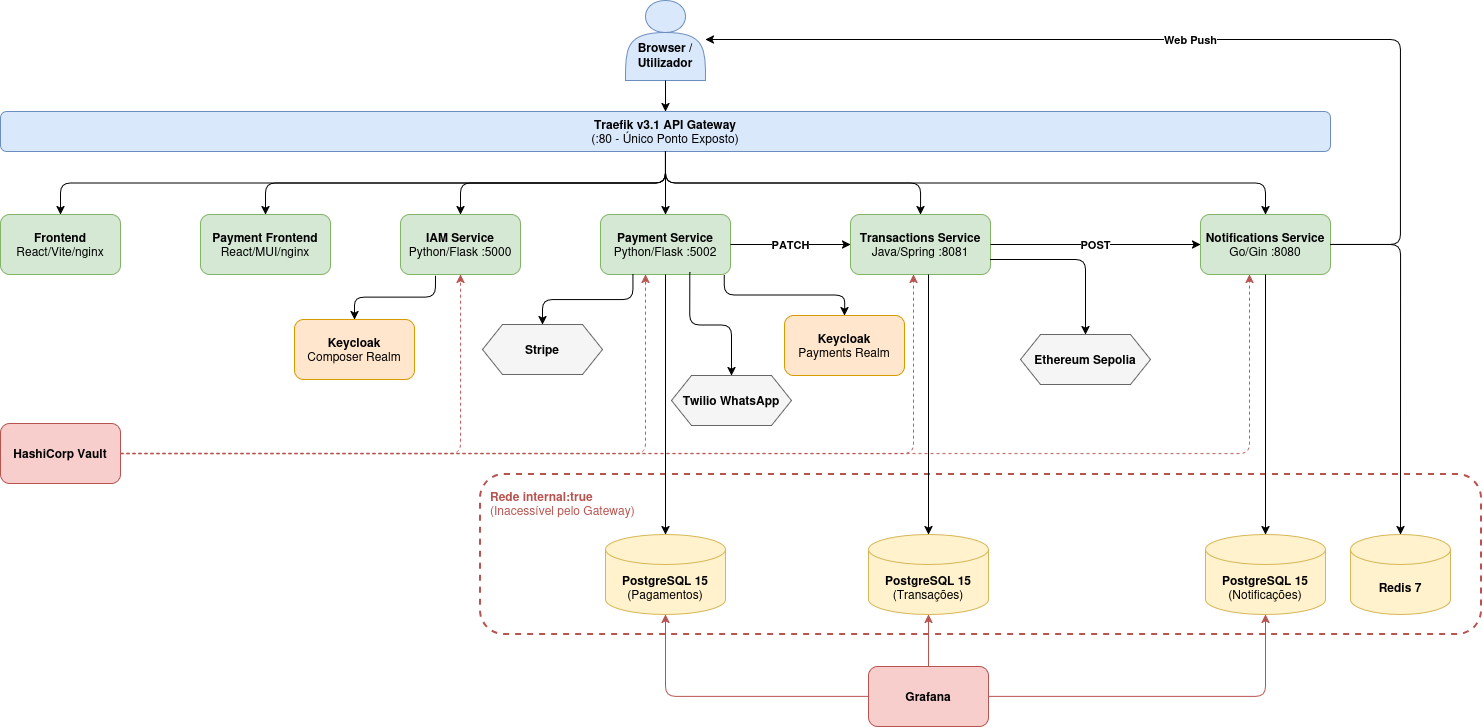
\includegraphics[width=\linewidth]{EGS_GERAL_ARCH.png}
  \caption{Arquitetura Geral do Sistema}
  \label{fig:arch}
\end{figure}

O roteamento do \emph{gateway} Traefik é baseado em \emph{headers} de \emph{host} HTTP,
conforme indicado na Tabela~\ref{tab:routing}.

\begin{table}[H]
\centering
\caption{Roteamento via Traefik (desenvolvimento local)}
\label{tab:routing}
\begin{tabularx}{\linewidth}{@{}L{5cm}L{5cm}C{2.5cm}@{}}
\toprule
\textbf{Host} & \textbf{Serviço} & \textbf{Porta interna} \\
\midrule
\texttt{app.pt}              & Frontend principal      & 80    \\
\texttt{payment.pt}          & Payment frontend        & 5174  \\
\texttt{iam.pt}              & IAM service             & 5000  \\
\texttt{transactions.pt}     & Transactions service    & 8081  \\
\texttt{payment-api.pt}      & Payment backend         & 5002  \\
\texttt{notifications.pt}    & Notifications service   & 8080  \\
\texttt{keycloak.pt}         & Keycloak (compositor)   & 8080  \\
\texttt{payment-keycloak.pt} & Keycloak (pagamentos)   & 8080  \\
\texttt{grafana.pt}          & Grafana                 & 3000  \\
\bottomrule
\end{tabularx}
\end{table}

% ============================================================
\section{Arquitetura de Microserviços}
\label{sec:arquitetura}

\subsection{Princípios Aplicados}

A arquitetura do PayNexus foi desenhada com os princípios fundamentais de microserviços
em mente. A Tabela~\ref{tab:principios} descreve como cada princípio foi concretizado
no projeto.

\begin{table}[H]
\centering
\caption{Princípios de microserviços e aplicação no projeto}
\label{tab:principios}
\begin{tabularx}{\linewidth}{@{}L{4cm}X@{}}
\toprule
\textbf{Princípio} & \textbf{Aplicação no PayNexus} \\
\midrule
\emph{Bounded contexts} & Cada serviço possui um domínio exclusivo: identidade, pagamentos, transações, notificações \\
Implantação independente & Cada serviço tem o seu próprio \texttt{Dockerfile}, imagem e ciclo de vida \\
Desenvolvimento políglota & Python (APIs web rápidas), Java/Spring (blockchain + tipagem forte), Go (notificações de alto débito) \\
Base de dados por serviço & Sem esquema partilhado; instância PostgreSQL isolada por serviço em rede própria \\
Isolamento de falhas & Uma falha no serviço de notificações não afeta os pagamentos \\
Ponto de entrada único & O Traefik esconde a topologia interna atrás de uma única porta \\
\bottomrule
\end{tabularx}
\end{table}

\textbf{Trade-offs aceites:} a abordagem microserviços introduz maior complexidade
operacional (muitos contentores, muitos segredos), consistência eventual entre serviços
(o pagamento só é ``concluído'' após o \emph{webhook} da Stripe, não quando o utilizador
clica), e autenticação inter-serviços que num monolito não seria necessária.

\subsection{Catálogo de Serviços}

A Tabela~\ref{tab:catalogo} apresenta o catálogo completo dos seis serviços que compõem
a plataforma.

\begin{longtable}{@{}L{2.8cm}L{3.5cm}L{2.5cm}C{1.2cm}L{3.2cm}@{}}
\caption{Catálogo de microserviços do PayNexus}
\label{tab:catalogo}\\
\toprule
\textbf{Serviço} & \textbf{Responsabilidade} & \textbf{Framework} & \textbf{Porta} & \textbf{Bibliotecas-chave} \\
\midrule
\endfirsthead
\multicolumn{5}{l}{\small\textit{(continuação da Tabela~\ref{tab:catalogo})}}\\
\toprule
\textbf{Serviço} & \textbf{Responsabilidade} & \textbf{Framework} & \textbf{Porta} & \textbf{Bibliotecas-chave} \\
\midrule
\endhead
\bottomrule
\endfoot
iam\_service & Registo, login e validação de \emph{tokens} via Keycloak & Python/Flask 3.1 & 5000 & python-keycloak, Flask \\[4pt]
payment\_service & Pagamentos com cartão, OTP, recibos, cartões guardados & Python/Flask 3.1 & 5002 & Stripe 14.4, Twilio, SQLAlchemy, ReportLab \\[4pt]
transactions\_service & Carteiras, transações \emph{blockchain}, composição BFF & Java 21/Spring Boot 3.4.3 & 8081 & Web3j 4.10, Spring Data JPA, SpringDoc \\[4pt]
notifications\_service & Clientes, subscrições, Web Push em tempo real & Go/Gin & 8080 & gin, gorm, webpush-go, jwt \\[4pt]
frontend & UI principal da carteira e histórico & React 18 + TypeScript + Vite & 80 & React Router, Axios, React Query \\[4pt]
payment frontend & UI de pagamento dedicada & React 18 + TypeScript + MUI & 5174 & @stripe/react-stripe-js, MUI \\
\end{longtable}

% ============================================================
\section{Stack Tecnológica}
\label{sec:stack}

A Tabela~\ref{tab:stack} resume todas as tecnologias utilizadas na plataforma, organizadas
por camada funcional.

\begin{longtable}{@{}L{3cm}L{4cm}L{5.5cm}@{}}
\caption{Stack tecnológica completa do PayNexus}
\label{tab:stack}\\
\toprule
\textbf{Camada} & \textbf{Tecnologia} & \textbf{Versão / Notas} \\
\midrule
\endfirsthead
\multicolumn{3}{l}{\small\textit{(continuação da Tabela~\ref{tab:stack})}}\\
\toprule
\textbf{Camada} & \textbf{Tecnologia} & \textbf{Versão / Notas} \\
\midrule
\endhead
\bottomrule
\endfoot
\emph{Frontend} & React + TypeScript + Vite & React 18.2, Vite 5.5, servido via nginx \\
 & Material-UI (MUI) & 7.3.9 --- biblioteca de componentes UI \\
 & Axios, React Query, React Router & HTTP, \emph{data fetching}, roteamento \\[4pt]
\emph{Backend} & Python 3.11 + Flask 3.1 & IAM e Payment services \\
 & Java 21 + Spring Boot & Transactions service (versão 3.4.3) \\
 & Go + Gin 1.10 & Notifications service \\[4pt]
Dados & PostgreSQL 15 & Uma instância por serviço \\
 & Redis 7 & Notificações --- cache e pub/sub \\
 & ORMs & SQLAlchemy, Spring Data JPA, GORM \\[4pt]
Autenticação & Keycloak 26.1 & Dois \emph{realms}, OAuth2/OIDC, JWT \\[4pt]
\emph{Gateway} & Traefik v3.1 & Roteamento por \emph{host}, multi-instância \\[4pt]
Contentores & Docker + Docker Compose & \emph{Multi-stage builds} \\
Orquestração & Kubernetes & Cluster DETI, Traefik Ingress \\[4pt]
Segredos & HashiCorp Vault 1.17 & AppRole + \emph{agent sidecars} \\[4pt]
Observabilidade & Grafana 10 & Datasources PostgreSQL por serviço \\[4pt]
Pagamentos & Stripe SDK 14.4.1 & PaymentIntent + \emph{webhooks} \\
OTP/SMS & Twilio SDK 9.10.4 & WhatsApp OTP \\
\emph{Blockchain} & Web3j 4.10 + Ethereum Sepolia & Chain ID: 11155111 \\
\emph{Push} & Web Push API + webpush-go & VAPID por cliente \emph{tenant} \\
\end{longtable}

% ============================================================
\section{Implementação dos Serviços}
\label{sec:servicos}

\subsection{IAM Service (Serviço de Identidade)}

O \textbf{IAM Service} é o ponto de entrada para autenticação de utilizadores. Implementado
em Python/Flask~3.1, funciona como um \emph{proxy} OIDC que delega toda a lógica de
identidade ao Keycloak.

\textbf{Responsabilidades:}
\begin{itemize}[noitemsep]
  \item Gerir o fluxo de \emph{sign-up} e \emph{login} via Keycloak (\emph{realm} compositor);
  \item Trocar o código de autorização OAuth2 por \emph{tokens} JWT;
  \item Validar \emph{tokens} em pedidos subsequentes;
  \item Expor documentação Swagger em \texttt{/iam/docs}.
\end{itemize}

A biblioteca \texttt{python-keycloak} abstrai a integração OIDC, e o estado de sessão
para validação do parâmetro \texttt{state} do OAuth2 é mantido em sistema de ficheiros.

\subsection{Payment Service (Serviço de Pagamentos)}

O \textbf{Payment Service}, implementado em Python/Flask~3.1 com SQLAlchemy e
PostgreSQL~15, é responsável por todo o ciclo de vida dos pagamentos com cartão.

\textbf{Fluxo principal:}
\begin{enumerate}[noitemsep]
  \item O \emph{frontend} invoca \texttt{POST /v1/payments} para criar um \texttt{PaymentIntent} na Stripe;
  \item O Stripe.js no browser confirma o pagamento diretamente com a Stripe;
  \item A Stripe envia um \emph{webhook} com assinatura HMAC para \texttt{POST /v1/payments/webhook};
  \item O serviço verifica a assinatura no cabeçalho \texttt{Stripe-Signature};
  \item É enviado um OTP de 6 dígitos via WhatsApp (Twilio), com validade de 5 minutos;
  \item Após verificação do OTP, o pagamento é marcado como \texttt{concluded} e o serviço
        chama o Transactions Service (Tabela~\ref{tab:endpoints-payment}).
\end{enumerate}

\begin{table}[H]
\centering
\caption{Endpoints principais do Payment Service}
\label{tab:endpoints-payment}
\begin{tabularx}{\linewidth}{@{}L{3.5cm}L{2cm}X@{}}
\toprule
\textbf{Endpoint} & \textbf{Método} & \textbf{Descrição} \\
\midrule
\texttt{/v1/payments} & POST & Cria PaymentIntent na Stripe \\
\texttt{/v1/payments} & GET & Lista pagamentos do utilizador (Bearer JWT) \\
\texttt{/v1/payments/\{id\}} & PATCH & Atualiza estado do pagamento \\
\texttt{/v1/payments/\{id\}/send-otp} & POST & Envia OTP via Twilio WhatsApp \\
\texttt{/v1/payments/\{id\}/verify} & POST & Valida código OTP \\
\texttt{/v1/payments/webhook} & POST & Recebe \emph{webhook} Stripe (HMAC) \\
\texttt{/v1/payments/\{id\}/receipt} & GET & Gera recibo PDF (ReportLab) \\
\texttt{/v1/users/profile} & GET/PUT & Perfil do utilizador \\
\texttt{/v1/users/cards} & GET/POST & Cartões guardados (Stripe Customer) \\
\bottomrule
\end{tabularx}
\end{table}

\textbf{Modelo de dados (PostgreSQL):} o serviço mantém quatro tabelas ---
\texttt{payments} (UUID, user\_id, montante, estado, stripe\_payment\_intent\_id,
wallet\_id), \texttt{user\_profiles} (stripe\_customer\_id, número de telefone),
\texttt{saved\_cards} (payment\_method\_id, last4, marca, validade) e
\texttt{payment\_otps} (código com hash SHA-256, expiração, flag de utilização).

\textbf{Geração de recibos PDF:} a biblioteca ReportLab gera recibos em memória
(\emph{in-memory}), com valores em EUR e tipografia Helvetica, servidos com
\texttt{Content-Disposition: attachment}.

\subsection{Transactions Service (Serviço de Transações e Blockchain)}

O \textbf{Transactions Service} é o serviço mais complexo da plataforma. Implementado em
Java~21 com Spring Boot~3.4.3, integra a \emph{blockchain} Ethereum e age
simultaneamente como serviço de carteiras, \emph{composer/BFF} e orquestrador do fluxo
de pagamento.

\textbf{Integração blockchain (Web3j~4.10):}
\begin{itemize}[noitemsep]
  \item \textbf{Rede:} Ethereum Sepolia testnet (chain ID: 11155111);
  \item \textbf{Carteiras:} criadas por utilizador, com chaves privadas encriptadas
        em AES com uma chave mestra (\texttt{MASTER\_KEY\_FOR\_WALLET} injetada via Vault);
  \item \textbf{Operações:} consulta de saldo, estimativa de \emph{gas}, envio de transações,
        cálculo de taxas;
  \item \textbf{Modos:} \emph{mock provider} para desenvolvimento, \emph{real provider} para produção.
\end{itemize}

\textbf{Papel de BFF (Backend for Frontend):} o serviço expõe os mesmos endpoints de
autenticação do IAM Service (delegando ao Payment Service), e gere o fluxo de
composição: criação de pagamento → crédito em carteira → emissão de evento de
notificação. A anotação \texttt{@EnableAsync} permite que operações \emph{blockchain}
e notificações sejam executadas de forma assíncrona.

\textbf{Endpoints principais:}
\begin{itemize}[noitemsep]
  \item \texttt{POST /v1/payments} --- cria pagamento e regista transação pendente;
  \item \texttt{PATCH /v1/payments/\{id\}} --- conclui pagamento, credita carteira,
        emite evento (chamado pelo Payment Service com cabeçalho \texttt{X-Internal-Key});
  \item \texttt{GET /v1/payments/\{id\}} --- consulta detalhes;
  \item Delegação de \texttt{/v1/pay/login} e \texttt{/v1/pay/signup} para o Payment Service.
\end{itemize}

\subsection{Notifications Service (Serviço de Notificações)}

O \textbf{Notifications Service} é um motor \emph{Web Push} multi-\emph{tenant} de uso
geral, implementado em Go com o \emph{framework} Gin. Qualquer aplicação cliente pode ser
integrada em tempo de execução, recebendo uma chave API e par de chaves VAPID próprias.

\textbf{Ciclo de vida de um cliente \emph{tenant}:}
\begin{enumerate}[noitemsep]
  \item Administrador cria cliente via \texttt{POST /v1/admin/clients};
  \item Sistema devolve chave API + chaves VAPID (pública e privada);
  \item O cliente usa a chave VAPID pública para subscrever utilizadores no browser;
  \item Subscrições são registadas em \texttt{POST /v1/events/subscribe};
  \item O Transactions Service publica eventos em \texttt{POST /v1/events} com \emph{Bearer API key};
  \item O serviço entrega notificações cifradas via Web Push ao \emph{Service Worker} do browser.
\end{enumerate}

\textbf{Performance:} o Redis~7 é usado para cache de clientes e subscrições, reduzindo
consultas à base de dados PostgreSQL nas operações de alta frequência. Os \emph{tokens} JWT
de subscrição têm validade de 15 minutos.

\textbf{Segurança multi-tenant:} cada cliente recebe o seu próprio par de chaves VAPID,
garantindo isolamento criptográfico entre \emph{tenants} e cumprindo a RFC~8292~\cite{rfc8292}.

\subsection{Frontends (React)}

A plataforma inclui dois \emph{frontends} independentes:

\textbf{Frontend principal} (\texttt{app.pt}): SPA React~18 + TypeScript + Vite que
expõe a carteira digital, histórico de transações, e gestão de conta. Comunica com o
Transactions Service (BFF) para todas as operações. Servido por nginx Alpine.

\textbf{Payment Frontend} (\texttt{payment.pt}): SPA dedicada ao fluxo de pagamento,
construída com React~18 + MUI~7.3 e integra o Stripe.js via
\texttt{@stripe/react-stripe-js}. Isolada num Keycloak \emph{realm} separado, garantindo
que credenciais de utilizadores de pagamento nunca se misturam com o \emph{realm}
compositor.

Ambos os \emph{frontends} usam \emph{multi-stage Docker builds} (nó de construção +
nginx de runtime) e são roteados pelo Traefik através de cabeçalhos de \emph{host}.

% ============================================================
\section{Comunicação Inter-Serviços}
\label{sec:comunicacao}

Todos os serviços comunicam via \textbf{REST/HTTP} sobre as redes internas Docker/Kubernetes.
São usados dois padrões de autenticação: \emph{tokens} \textbf{JWT Bearer} para chamadas
orientadas ao utilizador, e o cabeçalho \textbf{\texttt{X-Internal-Key}} para chamadas
de serviço-a-serviço que não devem expor credenciais de utilizador.

\begin{table}[H]
\centering
\caption{Chamadas inter-serviços no PayNexus}
\label{tab:interservice}
\begin{tabularx}{\linewidth}{@{}L{3.5cm}L{3cm}L{3cm}L{3cm}@{}}
\toprule
\textbf{Chamada} & \textbf{De → Para} & \textbf{Endpoint} & \textbf{Autenticação} \\
\midrule
Concluir pagamento & Payment → Transactions & \texttt{PATCH /v1/payments/\{id\}} & \texttt{X-Internal-Key} \\
Emitir evento & Transactions → Notifications & \texttt{POST /v1/events} & \texttt{Bearer <api-key>} \\
Login/tokens & Frontend → IAM → Keycloak & Fluxo OIDC code & OAuth2 \\
Entrega Web Push & Notifications → Browser & Web Push cifrado & Chaves VAPID \\
\emph{Webhook} Stripe & Stripe → Payment & \texttt{POST /v1/payments/webhook} & HMAC \texttt{Stripe-Signature} \\
\bottomrule
\end{tabularx}
\end{table}

Uma consequência arquitetural importante é a \textbf{consistência eventual}: um pagamento
só é marcado como ``concluído'' após o \emph{webhook} da Stripe ser recebido e
verificado --- não quando o utilizador clica em ``pagar''. Isto significa que o sistema
aceita um período de latência entre a ação do utilizador e a atualização de estado,
em troca de garantia criptográfica de que o pagamento foi efetivamente processado.

\begin{figure}[H]
  \centering
  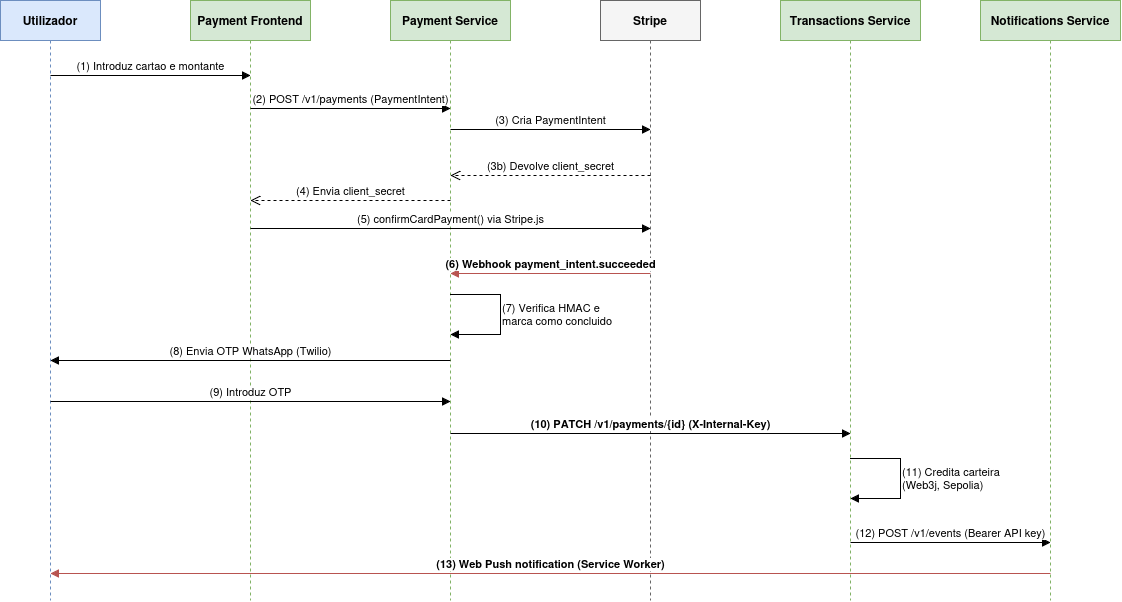
\includegraphics[width=0.95\linewidth]{EGS_SEQ_ADD_FUNDS.png}
  \caption{Diagrama de Sequência --- Fluxo de Pagamento e Carregamento de Carteira}
  \label{fig:seq-payment}
\end{figure}

% ============================================================
\section{Segurança}
\label{sec:seguranca}

A segurança do PayNexus é implementada em múltiplas camadas independentes, de forma a
que um eventual comprometimento de uma camada não exponha o sistema inteiro.

\subsection{Autenticação OAuth2/OIDC com Keycloak}

O Keycloak~26.1 é o provedor de identidade central da plataforma, configurado com
\textbf{dois \emph{realms} independentes}~\cite{keycloak,oauth2}:

\begin{itemize}[noitemsep]
  \item \textbf{\emph{Realm} compositor} (\texttt{keycloak.pt}): utilizado pela aplicação
        principal e pelo IAM Service para autenticar os utilizadores da carteira;
  \item \textbf{\emph{Realm} de pagamentos} (\texttt{payment-keycloak.pt}): utilizado
        exclusivamente pelo Payment Service, garantindo isolamento total entre os dois
        contextos de autenticação.
\end{itemize}

Esta separação implica que uma violação de credenciais no \emph{realm} de pagamentos não
compromete os utilizadores da carteira, e vice-versa. O custo é a duplicação de
configuração, mitigada pela exportação de \emph{realms} como ficheiros JSON versionados
(\texttt{realm-export.json}).

\begin{figure}[H]
  \centering
  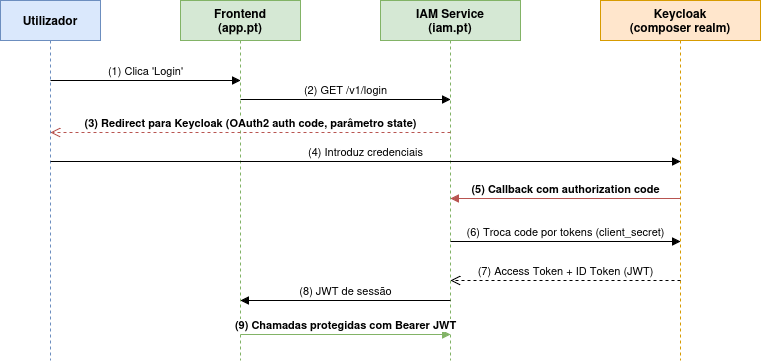
\includegraphics[width=0.95\linewidth]{EGS_SEQ_LOGIN.png}
  \caption{Fluxo de Login OIDC (OAuth2 Authorization Code Flow)}
  \label{fig:seq-login}
\end{figure}

\subsection{Gestão de Segredos com HashiCorp Vault}

Nenhum segredo é codificado na aplicação ou incluído nas imagens Docker. O HashiCorp
Vault~1.17~\cite{vault-approle,vault-agent} é o repositório centralizado de segredos,
com o padrão \textbf{AppRole + \emph{agent sidecar}}:

\begin{enumerate}[noitemsep]
  \item Cada serviço tem um \texttt{vault-agent} dedicado com \texttt{role\_id} e
        \texttt{secret\_id} próprios (AppRole);
  \item O agente autentica-se no Vault ao arrancar e renderiza o template
        \texttt{vault/templates/<serviço>.env.tmpl};
  \item O ficheiro \texttt{.env} resultante é montado em volume partilhado com o serviço;
  \item O processo do serviço lê as variáveis de ambiente sem nunca aceder diretamente
        ao Vault.
\end{enumerate}

\begin{table}[H]
\centering
\caption{Segredos geridos por serviço no Vault}
\label{tab:vault}
\begin{tabularx}{\linewidth}{@{}L{4cm}X@{}}
\toprule
\textbf{Serviço} & \textbf{Segredos injetados} \\
\midrule
payment\_service & \texttt{STRIPE\_SECRET\_KEY}, \texttt{STRIPE\_WEBHOOK\_SECRET}, \texttt{TWILIO\_ACCOUNT\_SID/AUTH\_TOKEN}, credenciais Keycloak, \texttt{DATABASE\_URL}, \texttt{INTERNAL\_API\_KEY} \\
transactions\_service & \texttt{MASTER\_KEY\_FOR\_WALLET} (AES), \texttt{NOTIFICATIONS\_API\_KEY}, \texttt{APP\_INTERNAL\_API\_KEY}, \texttt{BLOCKCHAIN\_NODE\_URL} \\
notifications\_service & \texttt{MASTER\_ADMIN\_SECRET}, \texttt{JWT\_SECRET}, \texttt{DATABASE\_URL} \\
iam\_service & \texttt{CLIENT\_SECRET} (Keycloak) \\
\emph{Bases de dados} & Passwords PostgreSQL por instância \\
\bottomrule
\end{tabularx}
\end{table}

\begin{figure}[H]
  \centering
  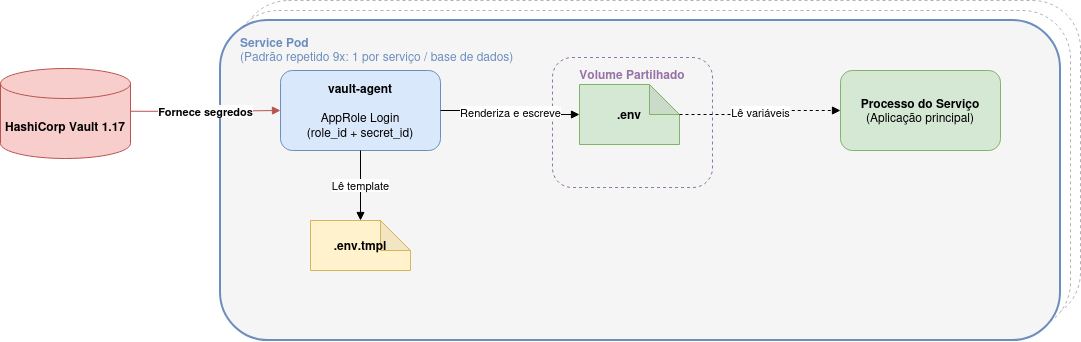
\includegraphics[width=0.85\linewidth]{EGS_Vault_diagram.png}
  \caption{Padrão Vault AppRole com Agent Sidecar}
  \label{fig:vault}
\end{figure}

\subsection{Outros Mecanismos de Segurança}

\begin{table}[H]
\centering
\caption{Mecanismos de segurança adicionais}
\label{tab:seguranca}
\begin{tabularx}{\linewidth}{@{}L{4.5cm}X@{}}
\toprule
\textbf{Mecanismo} & \textbf{Aplicação} \\
\midrule
RBAC (\emph{role} \texttt{operator}) & Endpoints de administração (estatísticas, criação de clientes) apenas acessíveis com papel \emph{operator} no JWT \\
Verificação HMAC \emph{webhook} & Cabeçalho \texttt{Stripe-Signature} verificado com a chave \texttt{STRIPE\_WEBHOOK\_SECRET} antes de processar qualquer evento \\
Encriptação AES de carteiras & Chaves privadas Ethereum encriptadas com \texttt{MASTER\_KEY\_FOR\_WALLET} antes de persistir na base de dados \\
OTP com hash SHA-256 & Código OTP armazenado apenas como hash; expiração de 5 minutos; flag \texttt{used} impede reutilização \\
Isolamento de rede & Redes de bases de dados com \texttt{internal: true} --- inacessíveis pelo Traefik ou pela rede pública \\
VAPID por \emph{tenant} & Isolamento criptográfico entre clientes nas notificações Web Push \\
\bottomrule
\end{tabularx}
\end{table}

% ============================================================
\section{Containerização e Orquestração}
\label{sec:containerizacao}

\subsection{Docker Compose (Desenvolvimento)}

Em desenvolvimento, a plataforma é orquestrada com Docker Compose num ficheiro raiz que
define \textbf{17 contentores}, 4 redes e 6 volumes nomeados~\cite{docker-multistage}.
Todos os serviços de aplicação usam \emph{multi-stage builds}:

\begin{table}[H]
\centering
\caption{Imagens Docker por serviço (\emph{multi-stage builds})}
\label{tab:docker}
\begin{tabularx}{\linewidth}{@{}L{4cm}L{4cm}L{4.5cm}@{}}
\toprule
\textbf{Serviço} & \textbf{Imagem de build} & \textbf{Imagem de runtime} \\
\midrule
Transactions (Java) & \texttt{maven:3.9-eclipse-temurin-21} & \texttt{eclipse-temurin:21-jre} \\
IAM / Payment (Python) & --- & \texttt{python:3.11-slim} \\
Notifications (Go) & \texttt{golang:alpine} & \texttt{alpine} \\
Frontends (React) & \texttt{node:20-slim} & \texttt{nginx:alpine} \\
\bottomrule
\end{tabularx}
\end{table}

\begin{figure}[H]
  \centering
  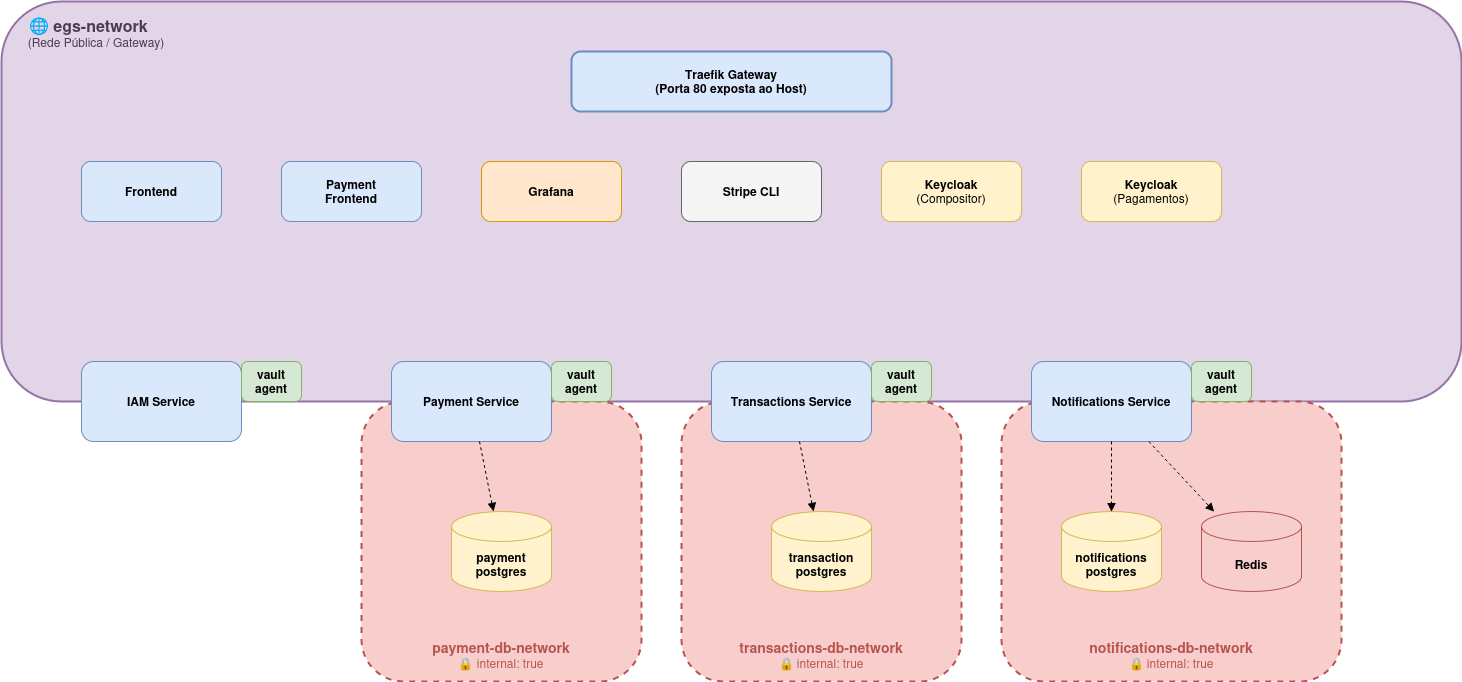
\includegraphics[width=\linewidth]{EGS_REDE_DOCKER.png}
  \caption{Topologia de Redes Docker Compose}
  \label{fig:docker-net}
\end{figure}

\subsection{Kubernetes (Produção)}

Em produção, a plataforma corre no cluster Kubernetes do DETI/UA, no namespace
\texttt{tenant-grupo3-egs-deti-ua-pt}~\cite{kubernetes}. Os manifestos disponíveis cobrem:

\begin{table}[H]
\centering
\caption{Manifestos Kubernetes disponíveis}
\label{tab:k8s-manifests}
\begin{tabularx}{\linewidth}{@{}L{5.5cm}X@{}}
\toprule
\textbf{Manifesto} & \textbf{Recursos definidos} \\
\midrule
\texttt{k8s/transactions-frontend.yaml} & Deployment (2 réplicas), ConfigMap (\texttt{VITE\_TRANSACTIONS\_BASE\_URL}), Service ClusterIP, Traefik Ingress (\texttt{transactions-frontend.grupo3-egs-deti-ua.pt}) \\
\texttt{k8s/notifications.yaml} & Notifications API Deployment (2 réplicas), PostgreSQL Deployment + PVC (1Gi), Redis Deployment, 4 Services ClusterIP, K8s Secret, Traefik Ingress (\texttt{notifications.grupo3-egs-deti-ua.pt}) \\
\texttt{k8s/grafana.yaml} & Grafana Deployment, 3 ConfigMaps (datasources, providers, 4 dashboards JSON embutidos), K8s Secret, Service, Traefik Ingress (\texttt{grafana.grupo3-egs-deti-ua.pt}) \\
\bottomrule
\end{tabularx}
\end{table}

A Tabela~\ref{tab:compose-vs-k8s} compara as duas estratégias de orquestração.

\begin{table}[H]
\centering
\caption{Docker Compose vs.\ Kubernetes}
\label{tab:compose-vs-k8s}
\begin{tabularx}{\linewidth}{@{}L{3cm}L{4.5cm}L{4.5cm}@{}}
\toprule
\textbf{Aspeto} & \textbf{Docker Compose} & \textbf{Kubernetes} \\
\midrule
Uso & Desenvolvimento local e demonstrações & Produção (cluster DETI) \\
Escalamento & Manual & Declarativo via \texttt{replicas} \\
Roteamento & Contentor Traefik & Traefik Ingress Controller \\
Segredos & Vault agents $\to$ \texttt{.env} & K8s Secrets \\
Armazenamento & Volumes nomeados & PersistentVolumeClaims \\
Âmbito & $\approx$17 contentores, um \emph{host} & Namespace, distribuído por nós \\
Limites de recursos & Não definidos & CPU/memória por contentor \\
\bottomrule
\end{tabularx}
\end{table}

% ============================================================
\section{Observabilidade}
\label{sec:observabilidade}

A observabilidade da plataforma é garantida pelo \textbf{Grafana~10}~\cite{grafana},
disponível em \texttt{grafana.pt} (desenvolvimento) e
\texttt{grafana.grupo3-egs-deti-ua.pt} (produção).

\textbf{Datasources:} três instâncias PostgreSQL independentes são configuradas como
fontes de dados --- uma por serviço com dados (transações, pagamentos, notificações).
A ausência de uma base de dados partilhada obriga a que cada dashboard consulte a sua
própria instância, refletindo a separação de domínios da arquitetura.

\textbf{Dashboards disponíveis:}
\begin{itemize}[noitemsep]
  \item \texttt{main\_dashboard}: visão global do sistema --- transações realizadas,
        notificações enviadas, pagamentos concluídos;
  \item \texttt{payments\_dashboard}: volume de pagamentos, receita, taxa de sucesso,
        estatísticas OTP, padrões horários (18 painéis);
  \item \texttt{transactions\_dashboard}: métricas \emph{blockchain} --- transações
        on-chain, saldos, taxas de gas;
  \item \texttt{notifications\_dashboard}: entrega de notificações, falhas, canais ativos.
\end{itemize}

\textbf{Provisionamento:} todos os datasources e dashboards são declarados como
configuração (ficheiros YAML e JSON), sem necessidade de configuração manual na UI.
Em Kubernetes, este provisionamento é encapsulado em ConfigMaps, garantindo que
o Grafana arranca totalmente configurado.

% ============================================================
\section{Desafios e Conclusões}
\label{sec:conclusao}

\subsection{Desafios Encontrados}

\begin{table}[H]
\centering
\caption{Desafios e aprendizagens do projeto}
\label{tab:desafios}
\begin{tabularx}{\linewidth}{@{}L{4.5cm}X@{}}
\toprule
\textbf{Desafio} & \textbf{Aprendizagem} \\
\midrule
Operações políglota & 4 linguagens = 4 cadeias de build/runtime para containerizar e manter consistentes \\
Segredos à escala & Vault + \emph{agent sidecars} eliminou segredos do código, mas acrescentou componentes móveis ao sistema \\
Dois \emph{realms} Keycloak & Isolamento forte entre utilizadores da carteira e do pagamento, ao custo de duplicação de configuração \\
Pagamentos por \emph{webhook} & Confiar nos \emph{webhooks} da Stripe (não no cliente) obriga a abraçar a consistência eventual \\
\emph{Testnet} Ethereum & Transações reais na Sepolia requerem \emph{gas}, encriptação de chaves e um \emph{mock provider} para desenvolvimento \\
\emph{Gateway} único & O Traefik simplificou a superfície de ataque --- uma porta exposta, tudo o resto interno \\
\bottomrule
\end{tabularx}
\end{table}

\subsection{Conclusões}

O projeto PayNexus demonstra que é viável implementar um sistema fintech com carregamento
direto de dinheiro para a \emph{blockchain} usando uma arquitetura de microserviços
políglota. A separação em \emph{bounded contexts} independentes permitiu usar a melhor
ferramenta para cada domínio: Python para APIs web rápidas, Java para a integração
\emph{blockchain} com tipagem forte, e Go para o motor de notificações de alto débito.

A segurança por camadas --- Keycloak, Vault, isolamento de rede, HMAC de \emph{webhooks},
e encriptação AES de chaves privadas --- garante que nenhum vetor de ataque isolado
compromete o sistema inteiro. A observabilidade com Grafana~10, aliada ao provisionamento
declarativo, torna o sistema operacionalmente maduro.

Do ponto de vista académico, o projeto cobre os temas centrais de Engenharia e Gestão de
Serviços: \emph{bounded contexts}, implantação independente, desenvolvimento políglota,
base de dados por serviço, \emph{API gateway}, segredos centralizados, e orquestração
com contentores em dois ambientes (Docker Compose e Kubernetes).

\textbf{Trabalho futuro:} integração de \emph{rate limiting} no Traefik, migração
completa para Kubernetes com Helm charts, adição de \emph{distributed tracing}
(OpenTelemetry), e extensão a redes Ethereum mainnet com \emph{fiat on-ramp} real.

% ============================================================
\bibliography{references}

\end{document}
